\hypertarget{group__dbprim__link}{
\section{Linked lists}
\label{group__dbprim__link}\index{Linked lists@{Linked lists}}
}


\subsection{Detailed Description}
Linked lists are a very basic data structure used in building databases. This library provides a simple yet powerful implementation of generic linked lists, based on two caller-allocated structures. The \hyperlink{group__dbprim__link_ga0}{link\_\-head\_\-t} structure describes the head of a linked list and contains information regarding the number of elements in the linked list as well as pointers referencing the first and last elements in the list. The \hyperlink{group__dbprim__link_ga1}{link\_\-elem\_\-t} structure describes a specific element in the linked list and contains pointers referencing the next and previous elements in the list, as well as a pointer to the object, a pointer to the head of the linked list, and a set of user-specified flags.

Elements may be added at any arbitrary location in the linked list with \hyperlink{group__dbprim__link_ga6}{ll\_\-add()}; moved to any other arbitrary location in the linked list with \hyperlink{group__dbprim__link_ga7}{ll\_\-move()}; or removed from the list with \hyperlink{group__dbprim__link_ga8}{ll\_\-remove()}. In addition, the user may search the list using a user-defined comparison function with \hyperlink{group__dbprim__link_ga9}{ll\_\-find()}; iterate over every element in the list with \hyperlink{group__dbprim__link_ga10}{ll\_\-iter()}; or remove all items from the list with \hyperlink{group__dbprim__link_ga11}{ll\_\-flush()}, optionally executing a user-specified clean-up function.

\subsection*{Data Structures}
\begin{CompactItemize}
\item 
struct \hyperlink{struct__link__head__s}{\_\-link\_\-head\_\-s}
\begin{CompactList}\small\item\em Linked list head structure. \item\end{CompactList}\item 
struct \hyperlink{struct__link__elem__s}{\_\-link\_\-elem\_\-s}
\begin{CompactList}\small\item\em Linked list element structure. \item\end{CompactList}\end{CompactItemize}
\subsection*{Defines}
\begin{CompactItemize}
\item 
\#define \hyperlink{group__dbprim__link_ga13}{LINK\_\-HEAD\_\-MAGIC}
\begin{CompactList}\small\item\em Linked list head magic number. \item\end{CompactList}\item 
\#define \hyperlink{group__dbprim__link_ga14}{LINK\_\-HEAD\_\-INIT}(extra)
\begin{CompactList}\small\item\em Linked list head static initializer. \item\end{CompactList}\item 
\#define \hyperlink{group__dbprim__link_ga15}{ll\_\-verify}(list)
\begin{CompactList}\small\item\em Linked list head verification macro. \item\end{CompactList}\item 
\#define \hyperlink{group__dbprim__link_ga16}{ll\_\-count}(list)
\begin{CompactList}\small\item\em Linked list count. \item\end{CompactList}\item 
\#define \hyperlink{group__dbprim__link_ga17}{ll\_\-first}(list)
\begin{CompactList}\small\item\em First element in linked list. \item\end{CompactList}\item 
\#define \hyperlink{group__dbprim__link_ga18}{ll\_\-last}(list)
\begin{CompactList}\small\item\em Last element in a linked list. \item\end{CompactList}\item 
\#define \hyperlink{group__dbprim__link_ga19}{ll\_\-extra}(list)
\begin{CompactList}\small\item\em Extra pointer data in a linked list. \item\end{CompactList}\item 
\#define \hyperlink{group__dbprim__link_ga20}{LINK\_\-ELEM\_\-MAGIC}
\begin{CompactList}\small\item\em Linked list element magic number. \item\end{CompactList}\item 
\#define \hyperlink{group__dbprim__link_ga21}{LINK\_\-ELEM\_\-INIT}(obj)
\begin{CompactList}\small\item\em Linked list element static initializer. \item\end{CompactList}\item 
\#define \hyperlink{group__dbprim__link_ga22}{le\_\-verify}(element)
\begin{CompactList}\small\item\em Linked list element verification macro. \item\end{CompactList}\item 
\#define \hyperlink{group__dbprim__link_ga23}{le\_\-next}(elem)
\begin{CompactList}\small\item\em Linked list element next pointer. \item\end{CompactList}\item 
\#define \hyperlink{group__dbprim__link_ga24}{le\_\-prev}(elem)
\begin{CompactList}\small\item\em Linked list element previous pointer. \item\end{CompactList}\item 
\#define \hyperlink{group__dbprim__link_ga25}{le\_\-object}(elem)
\begin{CompactList}\small\item\em Linked list element object pointer. \item\end{CompactList}\item 
\#define \hyperlink{group__dbprim__link_ga26}{le\_\-head}(elem)
\begin{CompactList}\small\item\em Linked list element head pointer. \item\end{CompactList}\item 
\#define \hyperlink{group__dbprim__link_ga27}{le\_\-flags}(elem)
\begin{CompactList}\small\item\em Linked list element flags. \item\end{CompactList}\end{CompactItemize}
\subsection*{Typedefs}
\begin{CompactItemize}
\item 
typedef \hyperlink{struct__link__head__s}{\_\-link\_\-head\_\-s} \hyperlink{group__dbprim__link_ga0}{link\_\-head\_\-t}
\begin{CompactList}\small\item\em Linked list head. \item\end{CompactList}\item 
typedef \hyperlink{struct__link__elem__s}{\_\-link\_\-elem\_\-s} \hyperlink{group__dbprim__link_ga1}{link\_\-elem\_\-t}
\begin{CompactList}\small\item\em Linked list element. \item\end{CompactList}\item 
typedef unsigned long($\ast$ \hyperlink{group__dbprim__link_ga2}{link\_\-iter\_\-t} )(\hyperlink{struct__link__head__s}{link\_\-head\_\-t} $\ast$list, \hyperlink{struct__link__elem__s}{link\_\-elem\_\-t} $\ast$elem, void $\ast$extra)
\begin{CompactList}\small\item\em Linked list iteration callback. \item\end{CompactList}\item 
typedef unsigned long($\ast$ \hyperlink{group__dbprim__link_ga3}{link\_\-comp\_\-t} )(\hyperlink{struct__db__key__s}{db\_\-key\_\-t} $\ast$key, void $\ast$obj)
\begin{CompactList}\small\item\em Linked list comparison callback. \item\end{CompactList}\item 
typedef enum \hyperlink{group__dbprim__link_ga28}{\_\-link\_\-loc\_\-e} \hyperlink{group__dbprim__link_ga4}{link\_\-loc\_\-t}
\begin{CompactList}\small\item\em Linked list location. \item\end{CompactList}\end{CompactItemize}
\subsection*{Enumerations}
\begin{CompactItemize}
\item 
enum \hyperlink{group__dbprim__link_ga28}{\_\-link\_\-loc\_\-e} \{ \hyperlink{group__dbprim__link_gga28a133}{LINK\_\-LOC\_\-HEAD}, 
\hyperlink{group__dbprim__link_gga28a134}{LINK\_\-LOC\_\-TAIL}, 
\hyperlink{group__dbprim__link_gga28a135}{LINK\_\-LOC\_\-BEFORE}, 
\hyperlink{group__dbprim__link_gga28a136}{LINK\_\-LOC\_\-AFTER}
 \}
\begin{CompactList}\small\item\em Linked list location. \item\end{CompactList}\end{CompactItemize}
\subsection*{Functions}
\begin{CompactItemize}
\item 
unsigned long \hyperlink{group__dbprim__link_ga5}{ll\_\-init} (\hyperlink{struct__link__head__s}{link\_\-head\_\-t} $\ast$list, void $\ast$extra)
\begin{CompactList}\small\item\em Dynamically initialize a linked list head. \item\end{CompactList}\item 
unsigned long \hyperlink{group__dbprim__link_ga6}{ll\_\-add} (\hyperlink{struct__link__head__s}{link\_\-head\_\-t} $\ast$list, \hyperlink{struct__link__elem__s}{link\_\-elem\_\-t} $\ast$new, \hyperlink{group__dbprim__link_ga4}{link\_\-loc\_\-t} loc, \hyperlink{struct__link__elem__s}{link\_\-elem\_\-t} $\ast$elem)
\begin{CompactList}\small\item\em Add an element to a linked list. \item\end{CompactList}\item 
unsigned long \hyperlink{group__dbprim__link_ga7}{ll\_\-move} (\hyperlink{struct__link__head__s}{link\_\-head\_\-t} $\ast$list, \hyperlink{struct__link__elem__s}{link\_\-elem\_\-t} $\ast$elem, \hyperlink{group__dbprim__link_ga4}{link\_\-loc\_\-t} loc, \hyperlink{struct__link__elem__s}{link\_\-elem\_\-t} $\ast$elem2)
\begin{CompactList}\small\item\em Move an element within a linked list. \item\end{CompactList}\item 
unsigned long \hyperlink{group__dbprim__link_ga8}{ll\_\-remove} (\hyperlink{struct__link__head__s}{link\_\-head\_\-t} $\ast$list, \hyperlink{struct__link__elem__s}{link\_\-elem\_\-t} $\ast$elem)
\begin{CompactList}\small\item\em Remove an element from a linked list. \item\end{CompactList}\item 
unsigned long \hyperlink{group__dbprim__link_ga9}{ll\_\-find} (\hyperlink{struct__link__head__s}{link\_\-head\_\-t} $\ast$list, \hyperlink{struct__link__elem__s}{link\_\-elem\_\-t} $\ast$$\ast$elem\_\-p, \hyperlink{group__dbprim__link_ga3}{link\_\-comp\_\-t} comp\_\-func, \hyperlink{struct__link__elem__s}{link\_\-elem\_\-t} $\ast$start, \hyperlink{struct__db__key__s}{db\_\-key\_\-t} $\ast$key)
\begin{CompactList}\small\item\em Find an element in a linked list. \item\end{CompactList}\item 
unsigned long \hyperlink{group__dbprim__link_ga10}{ll\_\-iter} (\hyperlink{struct__link__head__s}{link\_\-head\_\-t} $\ast$list, \hyperlink{struct__link__elem__s}{link\_\-elem\_\-t} $\ast$start, \hyperlink{group__dbprim__link_ga2}{link\_\-iter\_\-t} iter\_\-func, void $\ast$extra, unsigned long flags)
\begin{CompactList}\small\item\em Iterate over each entry in a linked list. \item\end{CompactList}\item 
unsigned long \hyperlink{group__dbprim__link_ga11}{ll\_\-flush} (\hyperlink{struct__link__head__s}{link\_\-head\_\-t} $\ast$list, \hyperlink{group__dbprim__link_ga2}{link\_\-iter\_\-t} flush\_\-func, void $\ast$extra)
\begin{CompactList}\small\item\em Flush a linked list. \item\end{CompactList}\item 
unsigned long \hyperlink{group__dbprim__link_ga12}{le\_\-init} (\hyperlink{struct__link__elem__s}{link\_\-elem\_\-t} $\ast$elem, void $\ast$object)
\begin{CompactList}\small\item\em Dynamically initialize a linked list element. \item\end{CompactList}\end{CompactItemize}


\subsection{Define Documentation}
\hypertarget{group__dbprim__link_ga27}{
\index{dbprim_link@{dbprim\_\-link}!le_flags@{le\_\-flags}}
\index{le_flags@{le\_\-flags}!dbprim_link@{dbprim\_\-link}}
\subsubsection[le\_\-flags]{\setlength{\rightskip}{0pt plus 5cm}\#define le\_\-flags(elem)}}
\label{group__dbprim__link_ga27}


This macro retrieves a set of user-defined flags associated with the element. It may be used as an lvalue to set those flags.

\begin{Desc}
\item[Parameters:]
\begin{description}
\item[\mbox{$\leftarrow$} {\em elem}]A pointer to a \hyperlink{group__dbprim__link_ga1}{link\_\-elem\_\-t}.\end{description}
\end{Desc}
\begin{Desc}
\item[Returns:]An {\tt unsigned long} containing the flags associated with the element.\end{Desc}


Definition at line 1003 of file dbprim.h.\hypertarget{group__dbprim__link_ga26}{
\index{dbprim_link@{dbprim\_\-link}!le_head@{le\_\-head}}
\index{le_head@{le\_\-head}!dbprim_link@{dbprim\_\-link}}
\subsubsection[le\_\-head]{\setlength{\rightskip}{0pt plus 5cm}\#define le\_\-head(elem)}}
\label{group__dbprim__link_ga26}


This macro retrieves a pointer to the head of the linked list that the element is in.

\begin{Desc}
\item[Parameters:]
\begin{description}
\item[\mbox{$\leftarrow$} {\em elem}]A pointer to a \hyperlink{group__dbprim__link_ga1}{link\_\-elem\_\-t}.\end{description}
\end{Desc}
\begin{Desc}
\item[Returns:]A pointer to a \hyperlink{group__dbprim__link_ga0}{link\_\-head\_\-t} representing the head of the linked list the element is in.\end{Desc}


Definition at line 990 of file dbprim.h.\hypertarget{group__dbprim__link_ga23}{
\index{dbprim_link@{dbprim\_\-link}!le_next@{le\_\-next}}
\index{le_next@{le\_\-next}!dbprim_link@{dbprim\_\-link}}
\subsubsection[le\_\-next]{\setlength{\rightskip}{0pt plus 5cm}\#define le\_\-next(elem)}}
\label{group__dbprim__link_ga23}


This macro retrieves a pointer to the next element in the linked list.

\begin{Desc}
\item[Parameters:]
\begin{description}
\item[\mbox{$\leftarrow$} {\em elem}]A pointer to a \hyperlink{group__dbprim__link_ga1}{link\_\-elem\_\-t}.\end{description}
\end{Desc}
\begin{Desc}
\item[Returns:]A pointer to a \hyperlink{group__dbprim__link_ga1}{link\_\-elem\_\-t} representing the next element in the linked list.\end{Desc}


Definition at line 950 of file dbprim.h.

Referenced by ht\_\-find(), and ht\_\-iter().\hypertarget{group__dbprim__link_ga25}{
\index{dbprim_link@{dbprim\_\-link}!le_object@{le\_\-object}}
\index{le_object@{le\_\-object}!dbprim_link@{dbprim\_\-link}}
\subsubsection[le\_\-object]{\setlength{\rightskip}{0pt plus 5cm}\#define le\_\-object(elem)}}
\label{group__dbprim__link_ga25}


This macro retrieves a pointer to the object represented by the element. It may be used as an lvalue to change the object pointed to. Care should be taken when using this feature.

\begin{Desc}
\item[Parameters:]
\begin{description}
\item[\mbox{$\leftarrow$} {\em elem}]A pointer to a \hyperlink{group__dbprim__link_ga1}{link\_\-elem\_\-t}.\end{description}
\end{Desc}
\begin{Desc}
\item[Returns:]A pointer to {\tt void} representing the object associated with the linked list element.\end{Desc}


Definition at line 977 of file dbprim.h.

Referenced by \_\-sh\_\-flush\_\-iter(), \_\-sh\_\-iter\_\-iter(), \_\-smat\_\-alloc(), \_\-smat\_\-free(), ht\_\-add(), ht\_\-find(), ht\_\-flush(), ht\_\-iter(), ht\_\-resize(), sh\_\-find(), smat\_\-cleanup(), and t\_\-iter().\hypertarget{group__dbprim__link_ga24}{
\index{dbprim_link@{dbprim\_\-link}!le_prev@{le\_\-prev}}
\index{le_prev@{le\_\-prev}!dbprim_link@{dbprim\_\-link}}
\subsubsection[le\_\-prev]{\setlength{\rightskip}{0pt plus 5cm}\#define le\_\-prev(elem)}}
\label{group__dbprim__link_ga24}


This macro retrieves a pointer to the previous element in the linked list.

\begin{Desc}
\item[Parameters:]
\begin{description}
\item[\mbox{$\leftarrow$} {\em elem}]A pointer to a \hyperlink{group__dbprim__link_ga1}{link\_\-elem\_\-t}.\end{description}
\end{Desc}
\begin{Desc}
\item[Returns:]A pointer to a \hyperlink{group__dbprim__link_ga1}{link\_\-elem\_\-t} representing the previous element in the linked list.\end{Desc}


Definition at line 963 of file dbprim.h.\hypertarget{group__dbprim__link_ga22}{
\index{dbprim_link@{dbprim\_\-link}!le_verify@{le\_\-verify}}
\index{le_verify@{le\_\-verify}!dbprim_link@{dbprim\_\-link}}
\subsubsection[le\_\-verify]{\setlength{\rightskip}{0pt plus 5cm}\#define le\_\-verify(element)}}
\label{group__dbprim__link_ga22}


This macro verifies that a given pointer actually does point to a linked list element.

\begin{Desc}
\item[Warning:]This macro evaluates the {\tt element} argument twice.\end{Desc}
\begin{Desc}
\item[Parameters:]
\begin{description}
\item[\mbox{$\leftarrow$} {\em element}]A pointer to a \hyperlink{group__dbprim__link_ga1}{link\_\-elem\_\-t}.\end{description}
\end{Desc}
\begin{Desc}
\item[Returns:]Boolean {\tt true} if {\tt element} is a valid linked list element or {\tt false} otherwise.\end{Desc}


Definition at line 936 of file dbprim.h.

Referenced by ll\_\-add(), ll\_\-find(), ll\_\-iter(), ll\_\-move(), and ll\_\-remove().\hypertarget{group__dbprim__link_ga21}{
\index{dbprim_link@{dbprim\_\-link}!LINK_ELEM_INIT@{LINK\_\-ELEM\_\-INIT}}
\index{LINK_ELEM_INIT@{LINK\_\-ELEM\_\-INIT}!dbprim_link@{dbprim\_\-link}}
\subsubsection[LINK\_\-ELEM\_\-INIT]{\setlength{\rightskip}{0pt plus 5cm}\#define LINK\_\-ELEM\_\-INIT(obj)}}
\label{group__dbprim__link_ga21}


This macro statically initializes a \hyperlink{group__dbprim__link_ga1}{link\_\-elem\_\-t}.

\begin{Desc}
\item[Parameters:]
\begin{description}
\item[\mbox{$\leftarrow$} {\em obj}]A pointer to {\tt void} representing the object associated with the element.\end{description}
\end{Desc}


Definition at line 921 of file dbprim.h.\hypertarget{group__dbprim__link_ga20}{
\index{dbprim_link@{dbprim\_\-link}!LINK_ELEM_MAGIC@{LINK\_\-ELEM\_\-MAGIC}}
\index{LINK_ELEM_MAGIC@{LINK\_\-ELEM\_\-MAGIC}!dbprim_link@{dbprim\_\-link}}
\subsubsection[LINK\_\-ELEM\_\-MAGIC]{\setlength{\rightskip}{0pt plus 5cm}\#define LINK\_\-ELEM\_\-MAGIC}}
\label{group__dbprim__link_ga20}


\begin{Desc}
\item[For internal use only.]
This is the magic number used for the linked list element structure.\end{Desc}


Definition at line 911 of file dbprim.h.

Referenced by le\_\-init().\hypertarget{group__dbprim__link_ga14}{
\index{dbprim_link@{dbprim\_\-link}!LINK_HEAD_INIT@{LINK\_\-HEAD\_\-INIT}}
\index{LINK_HEAD_INIT@{LINK\_\-HEAD\_\-INIT}!dbprim_link@{dbprim\_\-link}}
\subsubsection[LINK\_\-HEAD\_\-INIT]{\setlength{\rightskip}{0pt plus 5cm}\#define LINK\_\-HEAD\_\-INIT(extra)}}
\label{group__dbprim__link_ga14}


This macro statically initializes a \hyperlink{group__dbprim__link_ga0}{link\_\-head\_\-t}.

\begin{Desc}
\item[Parameters:]
\begin{description}
\item[\mbox{$\leftarrow$} {\em extra}]Extra pointer data that should be associated with the list head.\end{description}
\end{Desc}


Definition at line 661 of file dbprim.h.\hypertarget{group__dbprim__link_ga13}{
\index{dbprim_link@{dbprim\_\-link}!LINK_HEAD_MAGIC@{LINK\_\-HEAD\_\-MAGIC}}
\index{LINK_HEAD_MAGIC@{LINK\_\-HEAD\_\-MAGIC}!dbprim_link@{dbprim\_\-link}}
\subsubsection[LINK\_\-HEAD\_\-MAGIC]{\setlength{\rightskip}{0pt plus 5cm}\#define LINK\_\-HEAD\_\-MAGIC}}
\label{group__dbprim__link_ga13}


\begin{Desc}
\item[For internal use only.]
This is the magic number used for the linked list head structure.\end{Desc}


Definition at line 651 of file dbprim.h.

Referenced by ll\_\-init().\hypertarget{group__dbprim__link_ga16}{
\index{dbprim_link@{dbprim\_\-link}!ll_count@{ll\_\-count}}
\index{ll_count@{ll\_\-count}!dbprim_link@{dbprim\_\-link}}
\subsubsection[ll\_\-count]{\setlength{\rightskip}{0pt plus 5cm}\#define ll\_\-count(list)}}
\label{group__dbprim__link_ga16}


This macro retrieves the number of elements in a linked list.

\begin{Desc}
\item[Parameters:]
\begin{description}
\item[\mbox{$\leftarrow$} {\em list}]A pointer to a \hyperlink{group__dbprim__link_ga0}{link\_\-head\_\-t}.\end{description}
\end{Desc}
\begin{Desc}
\item[Returns:]An {\tt unsigned long} containing a count of the number of elements in the linked list.\end{Desc}


Definition at line 689 of file dbprim.h.

Referenced by \_\-smat\_\-alloc(), and smat\_\-freemem().\hypertarget{group__dbprim__link_ga19}{
\index{dbprim_link@{dbprim\_\-link}!ll_extra@{ll\_\-extra}}
\index{ll_extra@{ll\_\-extra}!dbprim_link@{dbprim\_\-link}}
\subsubsection[ll\_\-extra]{\setlength{\rightskip}{0pt plus 5cm}\#define ll\_\-extra(list)}}
\label{group__dbprim__link_ga19}


This macro retrieves the extra pointer data associated with a particular linked list.

\begin{Desc}
\item[Parameters:]
\begin{description}
\item[\mbox{$\leftarrow$} {\em list}]A pointer to a \hyperlink{group__dbprim__link_ga0}{link\_\-head\_\-t}.\end{description}
\end{Desc}
\begin{Desc}
\item[Returns:]A pointer to {\tt void}.\end{Desc}


Definition at line 723 of file dbprim.h.\hypertarget{group__dbprim__link_ga17}{
\index{dbprim_link@{dbprim\_\-link}!ll_first@{ll\_\-first}}
\index{ll_first@{ll\_\-first}!dbprim_link@{dbprim\_\-link}}
\subsubsection[ll\_\-first]{\setlength{\rightskip}{0pt plus 5cm}\#define ll\_\-first(list)}}
\label{group__dbprim__link_ga17}


This macro retrieves the first element in a linked list.

\begin{Desc}
\item[Parameters:]
\begin{description}
\item[\mbox{$\leftarrow$} {\em list}]A pointer to a \hyperlink{group__dbprim__link_ga0}{link\_\-head\_\-t}.\end{description}
\end{Desc}
\begin{Desc}
\item[Returns:]A pointer to a \hyperlink{group__dbprim__link_ga1}{link\_\-elem\_\-t}.\end{Desc}


Definition at line 700 of file dbprim.h.

Referenced by \_\-smat\_\-alloc(), ht\_\-find(), ht\_\-flush(), ht\_\-iter(), ht\_\-resize(), and smat\_\-cleanup().\hypertarget{group__dbprim__link_ga18}{
\index{dbprim_link@{dbprim\_\-link}!ll_last@{ll\_\-last}}
\index{ll_last@{ll\_\-last}!dbprim_link@{dbprim\_\-link}}
\subsubsection[ll\_\-last]{\setlength{\rightskip}{0pt plus 5cm}\#define ll\_\-last(list)}}
\label{group__dbprim__link_ga18}


This macro retrieves the last element in a linked list.

\begin{Desc}
\item[Parameters:]
\begin{description}
\item[\mbox{$\leftarrow$} {\em list}]A pointer to a \hyperlink{group__dbprim__link_ga0}{link\_\-head\_\-t}.\end{description}
\end{Desc}
\begin{Desc}
\item[Returns:]A pointer to a \hyperlink{group__dbprim__link_ga1}{link\_\-elem\_\-t}.\end{Desc}


Definition at line 711 of file dbprim.h.\hypertarget{group__dbprim__link_ga15}{
\index{dbprim_link@{dbprim\_\-link}!ll_verify@{ll\_\-verify}}
\index{ll_verify@{ll\_\-verify}!dbprim_link@{dbprim\_\-link}}
\subsubsection[ll\_\-verify]{\setlength{\rightskip}{0pt plus 5cm}\#define ll\_\-verify(list)}}
\label{group__dbprim__link_ga15}


This macro verifies that a given pointer actually does point to a linked list head.

\begin{Desc}
\item[Warning:]This macro evaluates the {\tt list} argument twice.\end{Desc}
\begin{Desc}
\item[Parameters:]
\begin{description}
\item[\mbox{$\leftarrow$} {\em list}]A pointer to a \hyperlink{group__dbprim__link_ga0}{link\_\-head\_\-t}.\end{description}
\end{Desc}
\begin{Desc}
\item[Returns:]Boolean {\tt true} if {\tt list} is a valid linked list head or {\tt false} otherwise.\end{Desc}


Definition at line 676 of file dbprim.h.

Referenced by ll\_\-add(), ll\_\-find(), ll\_\-flush(), ll\_\-iter(), ll\_\-move(), and ll\_\-remove().

\subsection{Typedef Documentation}
\hypertarget{group__dbprim__link_ga3}{
\index{dbprim_link@{dbprim\_\-link}!link_comp_t@{link\_\-comp\_\-t}}
\index{link_comp_t@{link\_\-comp\_\-t}!dbprim_link@{dbprim\_\-link}}
\subsubsection[link\_\-comp\_\-t]{\setlength{\rightskip}{0pt plus 5cm}typedef unsigned long($\ast$ \hyperlink{group__dbprim__link_ga3}{link\_\-comp\_\-t})(\hyperlink{struct__db__key__s}{db\_\-key\_\-t} $\ast$key, void $\ast$obj)}}
\label{group__dbprim__link_ga3}


This function pointer references a callback used by \hyperlink{group__dbprim__link_ga9}{ll\_\-find()}. It should return 0 if the entry passed as the second argument matches the key passed as the first argument.

\begin{Desc}
\item[Parameters:]
\begin{description}
\item[\mbox{$\leftarrow$} {\em key}]The database key being searched for. \item[\mbox{$\leftarrow$} {\em obj}]The object to compare with the key.\end{description}
\end{Desc}
\begin{Desc}
\item[Returns:]Zero if {\tt key} matches {\tt obj}, non-zero otherwise.\end{Desc}


Definition at line 357 of file dbprim.h.\hypertarget{group__dbprim__link_ga1}{
\index{dbprim_link@{dbprim\_\-link}!link_elem_t@{link\_\-elem\_\-t}}
\index{link_elem_t@{link\_\-elem\_\-t}!dbprim_link@{dbprim\_\-link}}
\subsubsection[link\_\-elem\_\-t]{\setlength{\rightskip}{0pt plus 5cm}typedef struct \hyperlink{struct__link__elem__s}{\_\-link\_\-elem\_\-s} \hyperlink{struct__link__elem__s}{link\_\-elem\_\-t}}}
\label{group__dbprim__link_ga1}


This structure represents a single element of a linked list.

Definition at line 269 of file dbprim.h.\hypertarget{group__dbprim__link_ga0}{
\index{dbprim_link@{dbprim\_\-link}!link_head_t@{link\_\-head\_\-t}}
\index{link_head_t@{link\_\-head\_\-t}!dbprim_link@{dbprim\_\-link}}
\subsubsection[link\_\-head\_\-t]{\setlength{\rightskip}{0pt plus 5cm}typedef struct \hyperlink{struct__link__head__s}{\_\-link\_\-head\_\-s} \hyperlink{struct__link__head__s}{link\_\-head\_\-t}}}
\label{group__dbprim__link_ga0}


This structure is the head of all linked lists maintained by this library.

Definition at line 262 of file dbprim.h.\hypertarget{group__dbprim__link_ga2}{
\index{dbprim_link@{dbprim\_\-link}!link_iter_t@{link\_\-iter\_\-t}}
\index{link_iter_t@{link\_\-iter\_\-t}!dbprim_link@{dbprim\_\-link}}
\subsubsection[link\_\-iter\_\-t]{\setlength{\rightskip}{0pt plus 5cm}typedef unsigned long($\ast$ \hyperlink{group__dbprim__link_ga2}{link\_\-iter\_\-t})(\hyperlink{struct__link__head__s}{link\_\-head\_\-t} $\ast$list, \hyperlink{struct__link__elem__s}{link\_\-elem\_\-t} $\ast$elem, void $\ast$extra)}}
\label{group__dbprim__link_ga2}


This function pointer references a callback used by \hyperlink{group__dbprim__link_ga10}{ll\_\-iter()} and \hyperlink{group__dbprim__link_ga11}{ll\_\-flush()}. It should return 0 for success. A non-zero return value will terminate the operation and will become the return value of the \hyperlink{group__dbprim__link_ga10}{ll\_\-iter()} or \hyperlink{group__dbprim__link_ga11}{ll\_\-flush()} call.

\begin{Desc}
\item[Parameters:]
\begin{description}
\item[\mbox{$\leftarrow$} {\em head}]A pointer to a \hyperlink{group__dbprim__link_ga0}{link\_\-head\_\-t}. \item[\mbox{$\leftarrow$} {\em elem}]A pointer to the \hyperlink{group__dbprim__link_ga1}{link\_\-elem\_\-t} being considered. \item[\mbox{$\leftarrow$} {\em extra}]A {\tt void} pointer passed to \hyperlink{group__dbprim__link_ga10}{ll\_\-iter()} or \hyperlink{group__dbprim__link_ga11}{ll\_\-flush()}.\end{description}
\end{Desc}
\begin{Desc}
\item[Returns:]Zero for success, or non-zero to terminate the iteration.\end{Desc}


Definition at line 342 of file dbprim.h.\hypertarget{group__dbprim__link_ga4}{
\index{dbprim_link@{dbprim\_\-link}!link_loc_t@{link\_\-loc\_\-t}}
\index{link_loc_t@{link\_\-loc\_\-t}!dbprim_link@{dbprim\_\-link}}
\subsubsection[link\_\-loc\_\-t]{\setlength{\rightskip}{0pt plus 5cm}typedef enum \hyperlink{group__dbprim__link_ga28}{\_\-link\_\-loc\_\-e} \hyperlink{group__dbprim__link_ga4}{link\_\-loc\_\-t}}}
\label{group__dbprim__link_ga4}


See the documentation for the enumeration \hyperlink{group__dbprim__link_ga28}{\_\-link\_\-loc\_\-e}.

Definition at line 537 of file dbprim.h.

\subsection{Enumeration Type Documentation}
\hypertarget{group__dbprim__link_ga28}{
\index{dbprim_link@{dbprim\_\-link}!_link_loc_e@{\_\-link\_\-loc\_\-e}}
\index{_link_loc_e@{\_\-link\_\-loc\_\-e}!dbprim_link@{dbprim\_\-link}}
\subsubsection[\_\-link\_\-loc\_\-e]{\setlength{\rightskip}{0pt plus 5cm}enum \hyperlink{group__dbprim__link_ga28}{\_\-link\_\-loc\_\-e}}}
\label{group__dbprim__link_ga28}


This enumeration is used to specify where an element in a linked list should be placed. It should be referenced by the typedef \hyperlink{group__dbprim__link_ga4}{link\_\-loc\_\-t}.\begin{Desc}
\item[Enumerator: ]\par
\begin{description}
\index{LINK_LOC_HEAD@{LINK\_\-LOC\_\-HEAD}!dbprim_link@{dbprim\_\-link}}\index{dbprim_link@{dbprim\_\-link}!LINK_LOC_HEAD@{LINK\_\-LOC\_\-HEAD}}\item[{\em 
\hypertarget{group__dbprim__link_gga28a133}{
LINK\_\-LOC\_\-HEAD}
\label{group__dbprim__link_gga28a133}
}]Element should be inserted at head of list. \index{LINK_LOC_TAIL@{LINK\_\-LOC\_\-TAIL}!dbprim_link@{dbprim\_\-link}}\index{dbprim_link@{dbprim\_\-link}!LINK_LOC_TAIL@{LINK\_\-LOC\_\-TAIL}}\item[{\em 
\hypertarget{group__dbprim__link_gga28a134}{
LINK\_\-LOC\_\-TAIL}
\label{group__dbprim__link_gga28a134}
}]Element should be inserted at tail of list. \index{LINK_LOC_BEFORE@{LINK\_\-LOC\_\-BEFORE}!dbprim_link@{dbprim\_\-link}}\index{dbprim_link@{dbprim\_\-link}!LINK_LOC_BEFORE@{LINK\_\-LOC\_\-BEFORE}}\item[{\em 
\hypertarget{group__dbprim__link_gga28a135}{
LINK\_\-LOC\_\-BEFORE}
\label{group__dbprim__link_gga28a135}
}]Element should be inserted before specified element. \index{LINK_LOC_AFTER@{LINK\_\-LOC\_\-AFTER}!dbprim_link@{dbprim\_\-link}}\index{dbprim_link@{dbprim\_\-link}!LINK_LOC_AFTER@{LINK\_\-LOC\_\-AFTER}}\item[{\em 
\hypertarget{group__dbprim__link_gga28a136}{
LINK\_\-LOC\_\-AFTER}
\label{group__dbprim__link_gga28a136}
}]Element should be inserted after specified element. \end{description}
\end{Desc}



Definition at line 523 of file dbprim.h.

\subsection{Function Documentation}
\hypertarget{group__dbprim__link_ga12}{
\index{dbprim_link@{dbprim\_\-link}!le_init@{le\_\-init}}
\index{le_init@{le\_\-init}!dbprim_link@{dbprim\_\-link}}
\subsubsection[le\_\-init]{\setlength{\rightskip}{0pt plus 5cm}unsigned long le\_\-init (\hyperlink{struct__link__elem__s}{link\_\-elem\_\-t} $\ast$ {\em elem}, void $\ast$ {\em object})}}
\label{group__dbprim__link_ga12}


This function dynamically initializes a linked list element.

\begin{Desc}
\item[Parameters:]
\begin{description}
\item[\mbox{$\leftarrow$} {\em elem}]A pointer to a \hyperlink{group__dbprim__link_ga1}{link\_\-elem\_\-t} to be initialized. \item[\mbox{$\leftarrow$} {\em object}]A pointer to {\tt void} used to represent the object associated with the element.\end{description}
\end{Desc}
\begin{Desc}
\item[Return values:]
\begin{description}
\item[{\em DB\_\-ERR\_\-BADARGS}]A {\tt NULL} pointer was passed for {\tt elem} or {\tt object}.\end{description}
\end{Desc}


Definition at line 34 of file le\_\-init.c.

References \_\-link\_\-elem\_\-s::le\_\-flags, \_\-link\_\-elem\_\-s::le\_\-head, \_\-link\_\-elem\_\-s::le\_\-magic, \_\-link\_\-elem\_\-s::le\_\-next, \_\-link\_\-elem\_\-s::le\_\-object, \_\-link\_\-elem\_\-s::le\_\-prev, and LINK\_\-ELEM\_\-MAGIC.

Referenced by \_\-smat\_\-alloc(), he\_\-init(), and main().\hypertarget{group__dbprim__link_ga6}{
\index{dbprim_link@{dbprim\_\-link}!ll_add@{ll\_\-add}}
\index{ll_add@{ll\_\-add}!dbprim_link@{dbprim\_\-link}}
\subsubsection[ll\_\-add]{\setlength{\rightskip}{0pt plus 5cm}unsigned long ll\_\-add (\hyperlink{struct__link__head__s}{link\_\-head\_\-t} $\ast$ {\em list}, \hyperlink{struct__link__elem__s}{link\_\-elem\_\-t} $\ast$ {\em new}, \hyperlink{group__dbprim__link_ga4}{link\_\-loc\_\-t} {\em loc}, \hyperlink{struct__link__elem__s}{link\_\-elem\_\-t} $\ast$ {\em elem})}}
\label{group__dbprim__link_ga6}


This function adds a given element to a specified linked list in the specified location.

\begin{Desc}
\item[Parameters:]
\begin{description}
\item[\mbox{$\leftarrow$} {\em list}]A pointer to a \hyperlink{group__dbprim__link_ga0}{link\_\-head\_\-t}. \item[\mbox{$\leftarrow$} {\em new}]A pointer to the \hyperlink{group__dbprim__link_ga1}{link\_\-elem\_\-t} to be added to the linked list. \item[\mbox{$\leftarrow$} {\em loc}]A \hyperlink{group__dbprim__link_ga4}{link\_\-loc\_\-t} indicating where the entry should be added. \item[\mbox{$\leftarrow$} {\em elem}]A pointer to a \hyperlink{group__dbprim__link_ga1}{link\_\-elem\_\-t} describing another element in the list if {\tt loc} is \hyperlink{group__dbprim__link_gga28a135}{LINK\_\-LOC\_\-BEFORE} or \hyperlink{group__dbprim__link_gga28a136}{LINK\_\-LOC\_\-AFTER}.\end{description}
\end{Desc}
\begin{Desc}
\item[Return values:]
\begin{description}
\item[{\em DB\_\-ERR\_\-BADARGS}]An argument was invalid. \item[{\em DB\_\-ERR\_\-BUSY}]The element is already in a list. \item[{\em DB\_\-ERR\_\-WRONGTABLE}]{\tt elem} is in a different list. \item[{\em DB\_\-ERR\_\-UNUSED}]{\tt elem} is not in any list.\end{description}
\end{Desc}


Definition at line 34 of file ll\_\-add.c.

References \_\-link\_\-elem\_\-s::le\_\-head, \_\-link\_\-elem\_\-s::le\_\-next, \_\-link\_\-elem\_\-s::le\_\-prev, le\_\-verify, \_\-link\_\-head\_\-s::lh\_\-count, \_\-link\_\-head\_\-s::lh\_\-first, \_\-link\_\-head\_\-s::lh\_\-last, LINK\_\-LOC\_\-AFTER, LINK\_\-LOC\_\-BEFORE, LINK\_\-LOC\_\-HEAD, LINK\_\-LOC\_\-TAIL, and ll\_\-verify.

Referenced by \_\-smat\_\-free(), ht\_\-add(), ht\_\-move(), ht\_\-resize(), main(), and st\_\-add().\hypertarget{group__dbprim__link_ga9}{
\index{dbprim_link@{dbprim\_\-link}!ll_find@{ll\_\-find}}
\index{ll_find@{ll\_\-find}!dbprim_link@{dbprim\_\-link}}
\subsubsection[ll\_\-find]{\setlength{\rightskip}{0pt plus 5cm}unsigned long ll\_\-find (\hyperlink{struct__link__head__s}{link\_\-head\_\-t} $\ast$ {\em list}, \hyperlink{struct__link__elem__s}{link\_\-elem\_\-t} $\ast$$\ast$ {\em elem\_\-p}, \hyperlink{group__dbprim__link_ga3}{link\_\-comp\_\-t} {\em comp\_\-func}, \hyperlink{struct__link__elem__s}{link\_\-elem\_\-t} $\ast$ {\em start}, \hyperlink{struct__db__key__s}{db\_\-key\_\-t} $\ast$ {\em key})}}
\label{group__dbprim__link_ga9}


This function iterates through a linked list looking for an element that matches the given {\tt key}.

\begin{Desc}
\item[Parameters:]
\begin{description}
\item[\mbox{$\leftarrow$} {\em list}]A pointer to a \hyperlink{group__dbprim__link_ga0}{link\_\-head\_\-t}. \item[\mbox{$\rightarrow$} {\em elem\_\-p}]A pointer to a pointer to a \hyperlink{group__dbprim__link_ga1}{link\_\-elem\_\-t}. {\tt NULL} is an invalid value. \item[\mbox{$\leftarrow$} {\em comp\_\-func}]A pointer to a comparison function used to compare the key to a particular element. See the documentation for \hyperlink{group__dbprim__link_ga3}{link\_\-comp\_\-t} for more information. \item[\mbox{$\leftarrow$} {\em start}]A pointer to a \hyperlink{group__dbprim__link_ga1}{link\_\-elem\_\-t} describing where in the linked list to start. If {\tt NULL} is passed, the beginning of the list will be assumed. \item[\mbox{$\leftarrow$} {\em key}]A key to search for.\end{description}
\end{Desc}
\begin{Desc}
\item[Return values:]
\begin{description}
\item[{\em DB\_\-ERR\_\-BADARGS}]An argument was invalid. \item[{\em DB\_\-ERR\_\-WRONGTABLE}]{\tt start} is not in this linked list. \item[{\em DB\_\-ERR\_\-NOENTRY}]No matching entry was found.\end{description}
\end{Desc}


Definition at line 34 of file ll\_\-find.c.

References \_\-link\_\-elem\_\-s::le\_\-head, \_\-link\_\-elem\_\-s::le\_\-next, \_\-link\_\-elem\_\-s::le\_\-object, le\_\-verify, \_\-link\_\-head\_\-s::lh\_\-first, and ll\_\-verify.

Referenced by main(), and sh\_\-find().\hypertarget{group__dbprim__link_ga11}{
\index{dbprim_link@{dbprim\_\-link}!ll_flush@{ll\_\-flush}}
\index{ll_flush@{ll\_\-flush}!dbprim_link@{dbprim\_\-link}}
\subsubsection[ll\_\-flush]{\setlength{\rightskip}{0pt plus 5cm}unsigned long ll\_\-flush (\hyperlink{struct__link__head__s}{link\_\-head\_\-t} $\ast$ {\em list}, \hyperlink{group__dbprim__link_ga2}{link\_\-iter\_\-t} {\em flush\_\-func}, void $\ast$ {\em extra})}}
\label{group__dbprim__link_ga11}


This function flushes a linked list--that is, it removes each element from the list. If a {\tt flush\_\-func} is specified, it will be called on the entry after it has been removed from the list, and may safely call {\tt free()}.

\begin{Desc}
\item[Parameters:]
\begin{description}
\item[\mbox{$\leftarrow$} {\em list}]A pointer to a \hyperlink{group__dbprim__link_ga0}{link\_\-head\_\-t}. \item[\mbox{$\leftarrow$} {\em flush\_\-func}]A pointer to a callback function used to perform user-specified actions on an element after removing it from the list. May be {\tt NULL}. See the documentation for \hyperlink{group__dbprim__link_ga2}{link\_\-iter\_\-t} for more information. \item[\mbox{$\leftarrow$} {\em extra}]A {\tt void} pointer that will be passed to {\tt flush\_\-func}.\end{description}
\end{Desc}
\begin{Desc}
\item[Return values:]
\begin{description}
\item[{\em DB\_\-ERR\_\-BADARGS}]An argument was invalid.\end{description}
\end{Desc}


Definition at line 34 of file ll\_\-flush.c.

References \_\-link\_\-head\_\-s::lh\_\-count, \_\-link\_\-head\_\-s::lh\_\-first, \_\-link\_\-head\_\-s::lh\_\-last, ll\_\-remove(), and ll\_\-verify.

Referenced by main(), and sh\_\-flush().

Here is the call graph for this function:\begin{figure}[H]
\begin{center}
\leavevmode
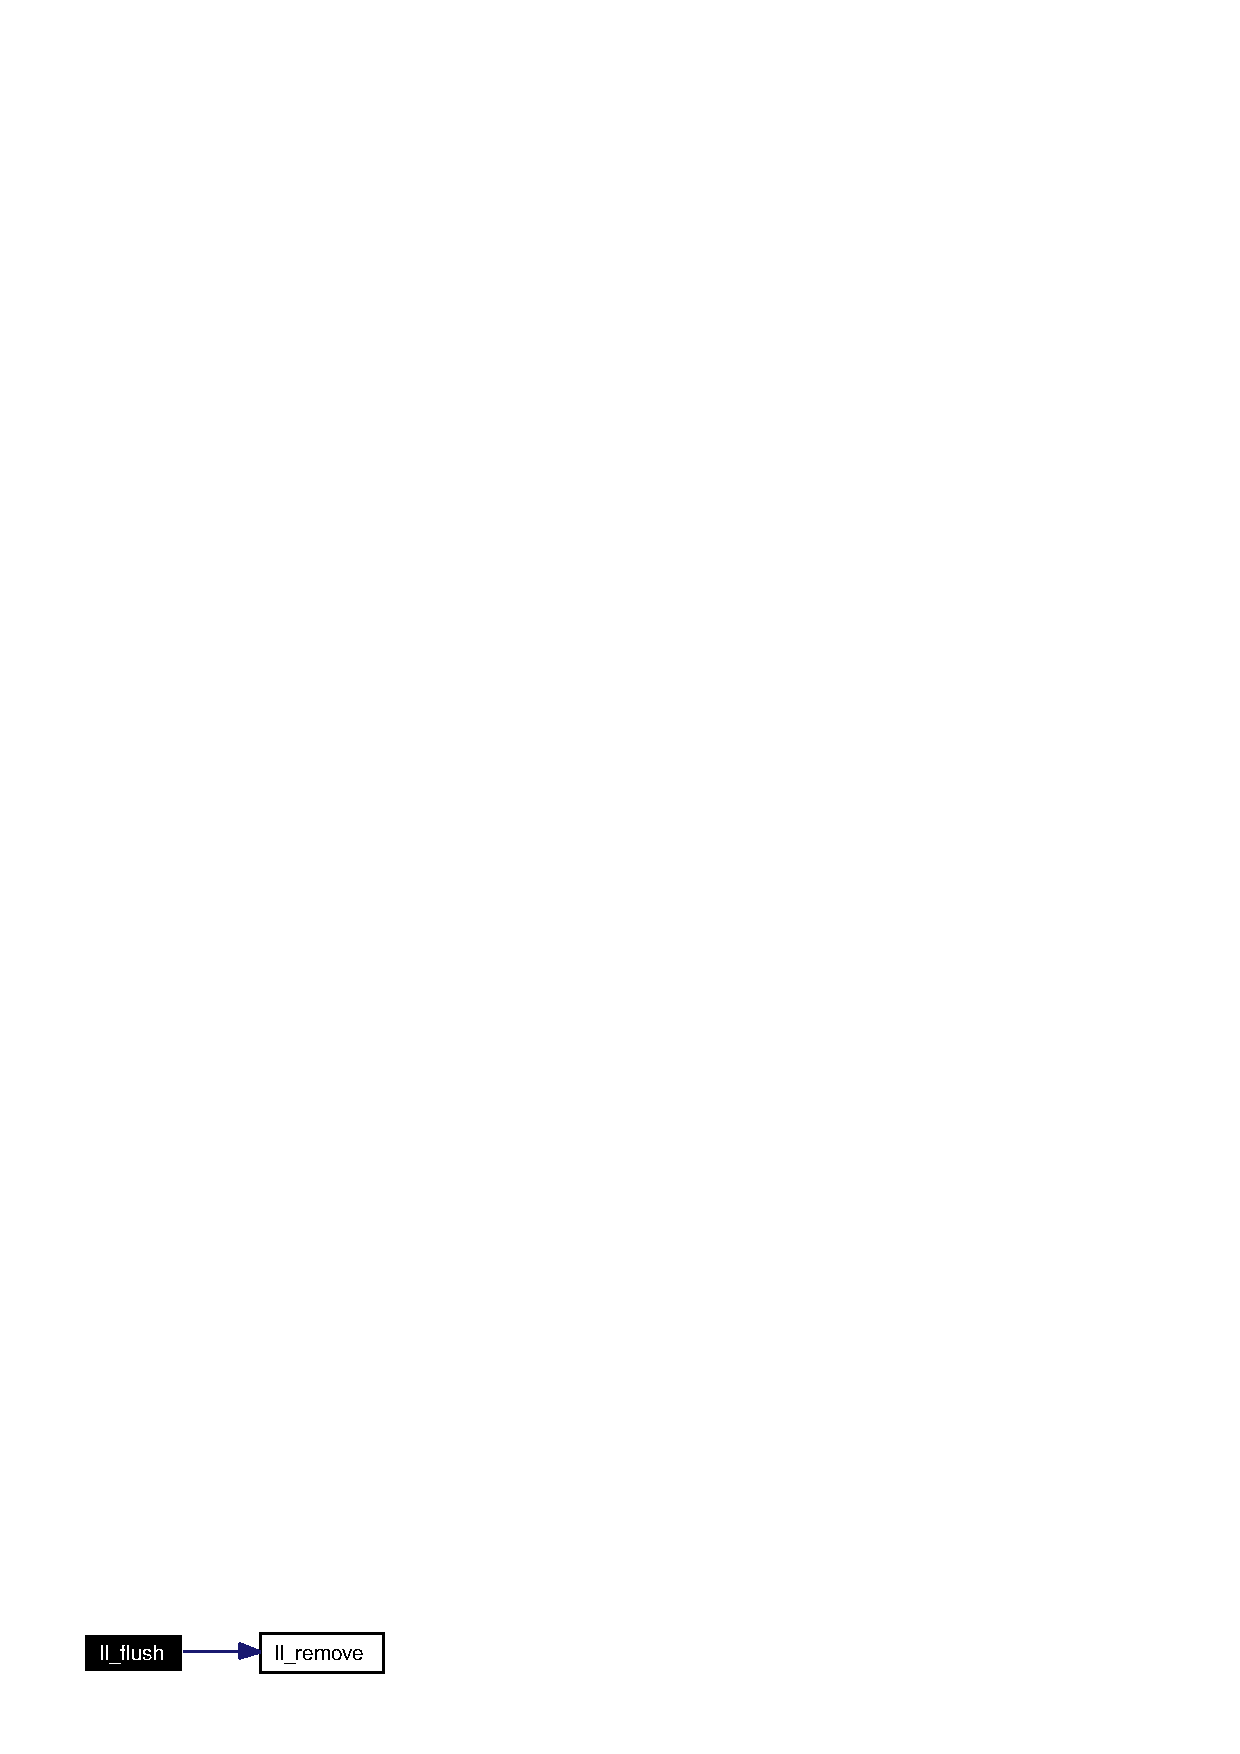
\includegraphics[width=94pt]{group__dbprim__link_ga11_cgraph}
\end{center}
\end{figure}
\hypertarget{group__dbprim__link_ga5}{
\index{dbprim_link@{dbprim\_\-link}!ll_init@{ll\_\-init}}
\index{ll_init@{ll\_\-init}!dbprim_link@{dbprim\_\-link}}
\subsubsection[ll\_\-init]{\setlength{\rightskip}{0pt plus 5cm}unsigned long ll\_\-init (\hyperlink{struct__link__head__s}{link\_\-head\_\-t} $\ast$ {\em list}, void $\ast$ {\em extra})}}
\label{group__dbprim__link_ga5}


This function dynamically initializes a linked list head.

\begin{Desc}
\item[Parameters:]
\begin{description}
\item[\mbox{$\leftarrow$} {\em list}]A pointer to a \hyperlink{group__dbprim__link_ga0}{link\_\-head\_\-t} to be initialized. \item[\mbox{$\leftarrow$} {\em extra}]A pointer to {\tt void} containing extra pointer data associated with the linked list.\end{description}
\end{Desc}
\begin{Desc}
\item[Return values:]
\begin{description}
\item[{\em DB\_\-ERR\_\-BADARGS}]A {\tt NULL} pointer was passed for {\tt list}.\end{description}
\end{Desc}


Definition at line 34 of file ll\_\-init.c.

References \_\-link\_\-head\_\-s::lh\_\-count, \_\-link\_\-head\_\-s::lh\_\-extra, \_\-link\_\-head\_\-s::lh\_\-first, \_\-link\_\-head\_\-s::lh\_\-last, \_\-link\_\-head\_\-s::lh\_\-magic, and LINK\_\-HEAD\_\-MAGIC.

Referenced by ht\_\-init(), ht\_\-resize(), main(), and sh\_\-init().\hypertarget{group__dbprim__link_ga10}{
\index{dbprim_link@{dbprim\_\-link}!ll_iter@{ll\_\-iter}}
\index{ll_iter@{ll\_\-iter}!dbprim_link@{dbprim\_\-link}}
\subsubsection[ll\_\-iter]{\setlength{\rightskip}{0pt plus 5cm}unsigned long ll\_\-iter (\hyperlink{struct__link__head__s}{link\_\-head\_\-t} $\ast$ {\em list}, \hyperlink{struct__link__elem__s}{link\_\-elem\_\-t} $\ast$ {\em start}, \hyperlink{group__dbprim__link_ga2}{link\_\-iter\_\-t} {\em iter\_\-func}, void $\ast$ {\em extra}, unsigned long {\em flags})}}
\label{group__dbprim__link_ga10}


This function iterates over a linked list, executing the given {\tt iter\_\-func} for each entry.

\begin{Desc}
\item[Parameters:]
\begin{description}
\item[\mbox{$\leftarrow$} {\em list}]A pointer to a \hyperlink{group__dbprim__link_ga0}{link\_\-head\_\-t}. \item[\mbox{$\leftarrow$} {\em start}]A pointer to a \hyperlink{group__dbprim__link_ga1}{link\_\-elem\_\-t} describing where in the linked list to start. If {\tt NULL} is passed, the beginning of the list will be assumed. \item[\mbox{$\leftarrow$} {\em iter\_\-func}]A pointer to a callback function used to perform user-specified actions on an element in a linked list. {\tt NULL} is an invalid value. See the documentation for \hyperlink{group__dbprim__link_ga2}{link\_\-iter\_\-t} for more information. \item[\mbox{$\leftarrow$} {\em extra}]A {\tt void} pointer that will be passed to {\tt iter\_\-func}. \item[\mbox{$\leftarrow$} {\em flags}]If \hyperlink{group__dbprim_ga4}{DB\_\-FLAG\_\-REVERSE} is given, iteration will be done from the end of the list backwards towards the head.\end{description}
\end{Desc}
\begin{Desc}
\item[Return values:]
\begin{description}
\item[{\em DB\_\-ERR\_\-BADARGS}]An argument was invalid. \item[{\em DB\_\-ERR\_\-WRONGTABLE}]{\tt start} is not in this linked list.\end{description}
\end{Desc}


Definition at line 34 of file ll\_\-iter.c.

References DB\_\-FLAG\_\-REVERSE, \_\-link\_\-elem\_\-s::le\_\-head, \_\-link\_\-elem\_\-s::le\_\-next, \_\-link\_\-elem\_\-s::le\_\-prev, le\_\-verify, \_\-link\_\-head\_\-s::lh\_\-first, \_\-link\_\-head\_\-s::lh\_\-last, and ll\_\-verify.

Referenced by main(), and sh\_\-iter().\hypertarget{group__dbprim__link_ga7}{
\index{dbprim_link@{dbprim\_\-link}!ll_move@{ll\_\-move}}
\index{ll_move@{ll\_\-move}!dbprim_link@{dbprim\_\-link}}
\subsubsection[ll\_\-move]{\setlength{\rightskip}{0pt plus 5cm}unsigned long ll\_\-move (\hyperlink{struct__link__head__s}{link\_\-head\_\-t} $\ast$ {\em list}, \hyperlink{struct__link__elem__s}{link\_\-elem\_\-t} $\ast$ {\em elem}, \hyperlink{group__dbprim__link_ga4}{link\_\-loc\_\-t} {\em loc}, \hyperlink{struct__link__elem__s}{link\_\-elem\_\-t} $\ast$ {\em elem2})}}
\label{group__dbprim__link_ga7}


This function moves a specified element within the linked list.

\begin{Desc}
\item[Parameters:]
\begin{description}
\item[\mbox{$\leftarrow$} {\em list}]A pointer to a \hyperlink{group__dbprim__link_ga0}{link\_\-head\_\-t}. \item[\mbox{$\leftarrow$} {\em elem}]A pointer to the \hyperlink{group__dbprim__link_ga1}{link\_\-elem\_\-t} describing the element to be moved. \item[\mbox{$\leftarrow$} {\em loc}]A \hyperlink{group__dbprim__link_ga4}{link\_\-loc\_\-t} indicating where the entry should be moved to. \item[\mbox{$\leftarrow$} {\em elem2}]A pointer to a \hyperlink{group__dbprim__link_ga1}{link\_\-elem\_\-t} describing another element in the list if {\tt loc} is \hyperlink{group__dbprim__link_gga28a135}{LINK\_\-LOC\_\-BEFORE} or \hyperlink{group__dbprim__link_gga28a136}{LINK\_\-LOC\_\-AFTER}.\end{description}
\end{Desc}
\begin{Desc}
\item[Return values:]
\begin{description}
\item[{\em DB\_\-ERR\_\-BADARGS}]An argument was invalid. \item[{\em DB\_\-ERR\_\-BUSY}]{\tt new} and {\tt elem} are the same element. \item[{\em DB\_\-ERR\_\-WRONGTABLE}]{\tt new} or {\tt elem} are in a different list. \item[{\em DB\_\-ERR\_\-UNUSED}]{\tt new} or {\tt elem} are not in any list.\end{description}
\end{Desc}


Definition at line 35 of file ll\_\-move.c.

References \_\-link\_\-elem\_\-s::le\_\-head, \_\-link\_\-elem\_\-s::le\_\-next, \_\-link\_\-elem\_\-s::le\_\-prev, le\_\-verify, \_\-link\_\-head\_\-s::lh\_\-first, \_\-link\_\-head\_\-s::lh\_\-last, LINK\_\-LOC\_\-AFTER, LINK\_\-LOC\_\-BEFORE, LINK\_\-LOC\_\-HEAD, LINK\_\-LOC\_\-TAIL, and ll\_\-verify.

Referenced by main(), and sh\_\-move().\hypertarget{group__dbprim__link_ga8}{
\index{dbprim_link@{dbprim\_\-link}!ll_remove@{ll\_\-remove}}
\index{ll_remove@{ll\_\-remove}!dbprim_link@{dbprim\_\-link}}
\subsubsection[ll\_\-remove]{\setlength{\rightskip}{0pt plus 5cm}unsigned long ll\_\-remove (\hyperlink{struct__link__head__s}{link\_\-head\_\-t} $\ast$ {\em list}, \hyperlink{struct__link__elem__s}{link\_\-elem\_\-t} $\ast$ {\em elem})}}
\label{group__dbprim__link_ga8}


This function removes a specified element from a linked list.

\begin{Desc}
\item[Parameters:]
\begin{description}
\item[\mbox{$\leftarrow$} {\em list}]A pointer to a \hyperlink{group__dbprim__link_ga0}{link\_\-head\_\-t}. \item[\mbox{$\leftarrow$} {\em elem}]A pointer to the \hyperlink{group__dbprim__link_ga1}{link\_\-elem\_\-t} describing the element to be removed.\end{description}
\end{Desc}
\begin{Desc}
\item[Return values:]
\begin{description}
\item[{\em DB\_\-ERR\_\-BADARGS}]An argument was invalid. \item[{\em DB\_\-ERR\_\-UNUSED}]{\tt elem} is not in a linked list. \item[{\em DB\_\-ERR\_\-WRONGTABLE}]{\tt elem} is not in this linked list.\end{description}
\end{Desc}


Definition at line 34 of file ll\_\-remove.c.

References \_\-link\_\-elem\_\-s::le\_\-head, \_\-link\_\-elem\_\-s::le\_\-next, \_\-link\_\-elem\_\-s::le\_\-prev, le\_\-verify, \_\-link\_\-head\_\-s::lh\_\-count, \_\-link\_\-head\_\-s::lh\_\-first, \_\-link\_\-head\_\-s::lh\_\-last, and ll\_\-verify.

Referenced by \_\-smat\_\-alloc(), \_\-st\_\-remove(), ht\_\-move(), ht\_\-remove(), ht\_\-resize(), ll\_\-flush(), main(), smat\_\-cleanup(), and st\_\-add().